\documentclass[leno,xcolor=dvipsnames]{beamer}
\usetheme{PaloAlto}           % Use metropolis theme

\usepackage{luatexja}% 日本語したい
\usepackage[ipaex]{luatexja-preset}% IPAexフォントしたい
\renewcommand{\kanjifamilydefault}{\gtdefault}% 既定をゴシック体に
\makeatletter
\newcommand{\figcaption}[1]{\def\@captype{figure}\caption{#1}}
\newcommand{\tblcaption}[1]{\def\@captype{table}\caption{#1}}
\makeatother

\usepackage{adjustbox}
\usepackage{float}
\usepackage{wrapfig}  % 図の回り込み
\usepackage{blindtext}
\usepackage{booktabs}
\usepackage{multirow}
\usepackage{ascmac}
\usepackage{fancybox}
\usepackage{amsmath}
\usepackage{mathtools}
\usepackage{siunitx}
\usepackage{tikz}
\usetikzlibrary {arrows.meta}
\usetikzlibrary {bending}
\usepackage{listings}
\lstset{
    frame={tb},
    basicstyle=\tiny\ttfamily,
    tabsize=4,
    numbers=left,
    breaklines=true,
    xleftmargin=1\zw,
    numberstyle={\scriptsize}
}

\title{進捗報告}
\date{\today}
\author{水野泰旭}
\institute{弘前大学理工学部電子情報工学科4年}
\begin{document}
  \maketitle
  % 目次
  \begin{frame}
    \frametitle{目次}
    \tableofcontents
  \end{frame}
  % 一章
  \section{F1スコア}
  \begin{frame}
    \frametitle{前回の問題点}
    \subsection{前回の問題点}
    \begin{columns}
      \begin{column}{0.48\textwidth}
          クラスDのTPとFPが共にゼロとなり、
          \[\mathrm{Precision} = \frac{\mathrm{TP}}{\mathrm{TP} + \mathrm{FP}}\]
          の値を取る適合率がゼロ除算となってしまう。現在は訓練データと検証データは9:1なので、8:2として学習してみる。
      \end{column}
      \begin{column}{0.48\textwidth}
        \begin{figure}[H]
          \centering
          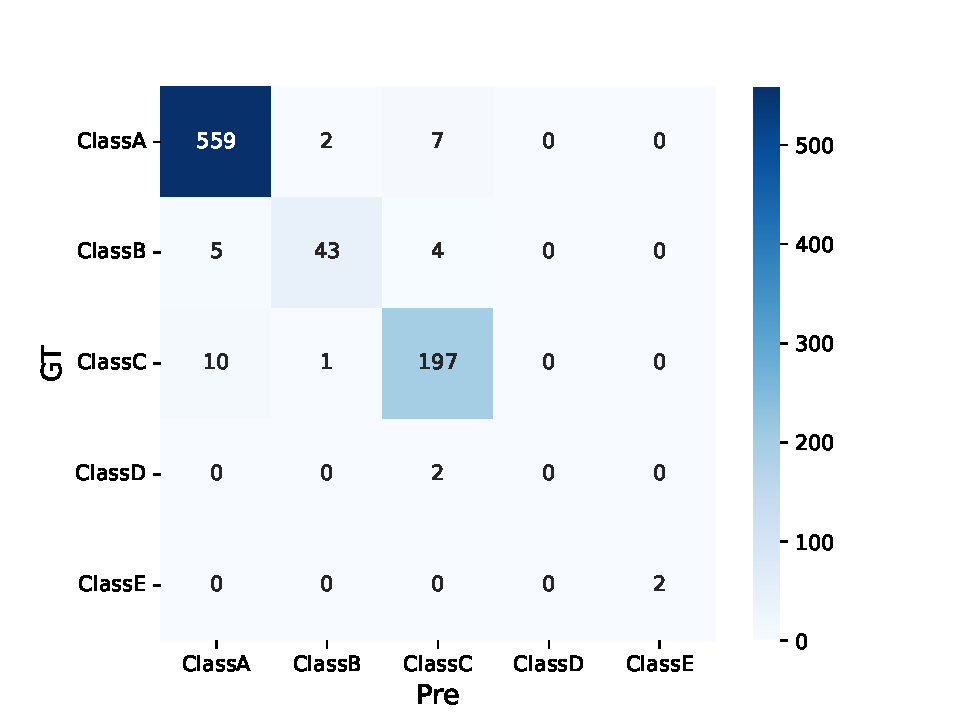
\includegraphics[keepaspectratio, scale=0.35]{images/deepimfam_confusion_matrix_cnt.pdf}
        \end{figure}
      \end{column}
    \end{columns}
  \end{frame}
  \begin{frame}
    \frametitle{検証データ20\%の混同行列}
    \subsection{検証データ20\%の混同行列}
    \begin{figure}[H]
      \centering
      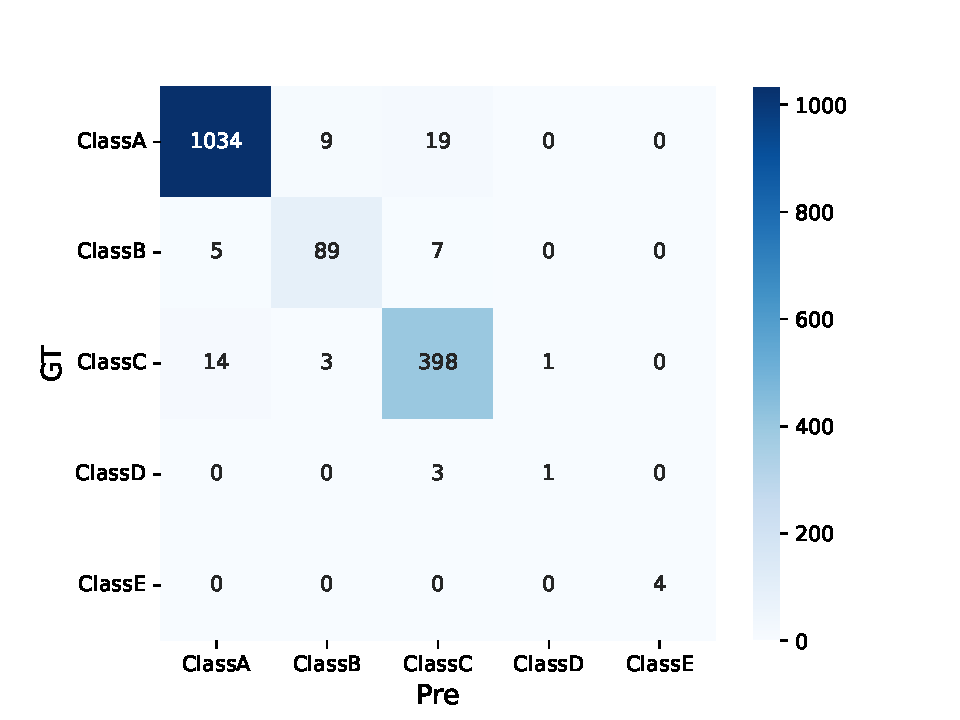
\includegraphics[keepaspectratio, scale=0.6]{images/DeepImFam_more_val.pdf}
    \end{figure}
  \end{frame}
  \begin{frame}
    \frametitle{Macro-F1スコアの再計算}
    \subsection{Macro-F1スコアの再計算}
    \begin{table}[H]
      \centering
      \caption{クラスごとのMacro-F1の計算} \label{tb:macro-F1}
      \begin{tabular}{ccccc}
        \toprule
        Class & Accuracy & Precision & Recall & Macro-F1 \\
        \midrule
        A & 0.97038 & 0.98195 & 0.97363 & 0.97777 \\
        B & 0.98487 & 0.88118 & 0.88118 & 0.88118 \\
        C & 0.97038 & 0.93208 & 0.95673 & 0.94424 \\
        D & 0.99810 & 1.00000 & 0.25000 & 0.40000 \\
        E & 1.00000 & 1.00000 & 1.00000 & 1.00000 \\
        \midrule
        Average & 0.98475 & 0.95904 & 0.81231 & 0.84064 \\
        \bottomrule
      \end{tabular}
    \end{table}
    sklearn.f1\_scoreでmacro-F1スコアの計算をすると、0.82730が出力され、手計算と異なる値となった。
  \end{frame}
  \section{データ数を揃えて学習}
  \begin{frame}[fragile]
    \frametitle{ソースコード}
    \subsection{ソースコード}
    画像の枚数が少ないクラスに対して、画像を適当な回数コピーしてだいたい同じ枚数にする。
    \begin{lstlisting}[caption=augmentation.py, language=Python]
# ラベルごとに抽出
index = list()
for i in range(5): index.append(train_labels == i)
each_train_images = dict()
each_train_labels = dict()
for i in range(5):
    each_train_images[i] = train_img[index[i]]
    each_train_labels[i] = train_labels[index[i]]

max_l = 0
for (key, val) in each_train_labels.items(): max_l = max(max_l, len(val))
augmentation_train_images = np.empty((0, 150, 150, 1))
augmentation_train_labels = np.empty(0)
for (key, val) in each_train_images.items():
    for i in range(max_l // len(val)):
        aug_train_images = np.append(aug_train_images, val, axis=0)
        aug_train_labels = np.append(aug_train_labels, each_train_labels[key])
    \end{lstlisting}
  \end{frame}
  \begin{frame}
    \frametitle{訓練データ数の推移}
    \subsection{訓練データ数の推移}
    \begin{columns}
      \begin{column}{0.48\textwidth}
        \begin{table}[H]
          \centering
          \caption{もとの訓練データ}
          \begin{tabular}{cr}
            \toprule
            クラス & データ数 \\
            \midrule
            A & 4824 \\
            B & 411 \\ 
            C & 1844 \\
            D & 11 \\
            E & 16 \\
            \midrule
            SUM & 7106 \\
            \bottomrule
          \end{tabular}
        \end{table}
      \end{column}
      \begin{column}{0.48\textwidth}
        \begin{table}[H]
          \centering
          \caption{増やした訓練データ}
          \begin{tabular}{cr}
            \toprule
            クラス & データ数 \\
            \midrule
            A & 4824 \\
            B & 4521 \\ 
            C & 3688 \\
            D & 4818 \\
            E & 4816 \\
            \midrule
            SUM & 22667 \\
            \bottomrule
          \end{tabular}
        \end{table}
      \end{column}
    \end{columns}
  \end{frame}
  \begin{frame}
    \frametitle{学習結果}
    \subsection{学習結果の比較}
    \begin{table}[H]
      \centering
      \caption{もとのデータと増やしたデータの学習結果}
      \begin{tabular}{rrr}
        \toprule
        & Accuracy & Macro-F1 \\
        \midrule
        もとのデータによる学習結果 & 0.9699 & 0.7598\footnote{クラスDのTPとFPが共にゼロとなりあまり正確ではない\\} \\
        水増しデータによる学習結果 & 0.9519 & 0.7656 \\ 
        \bottomrule
      \end{tabular}
    \end{table}
  \end{frame}
  \begin{frame}
    \frametitle{混同行列の比較}
    \frametitle{混同行列の比較}
    \begin{columns}
      \begin{column}{0.48\textwidth}
        \begin{figure}[H]
          \centering
          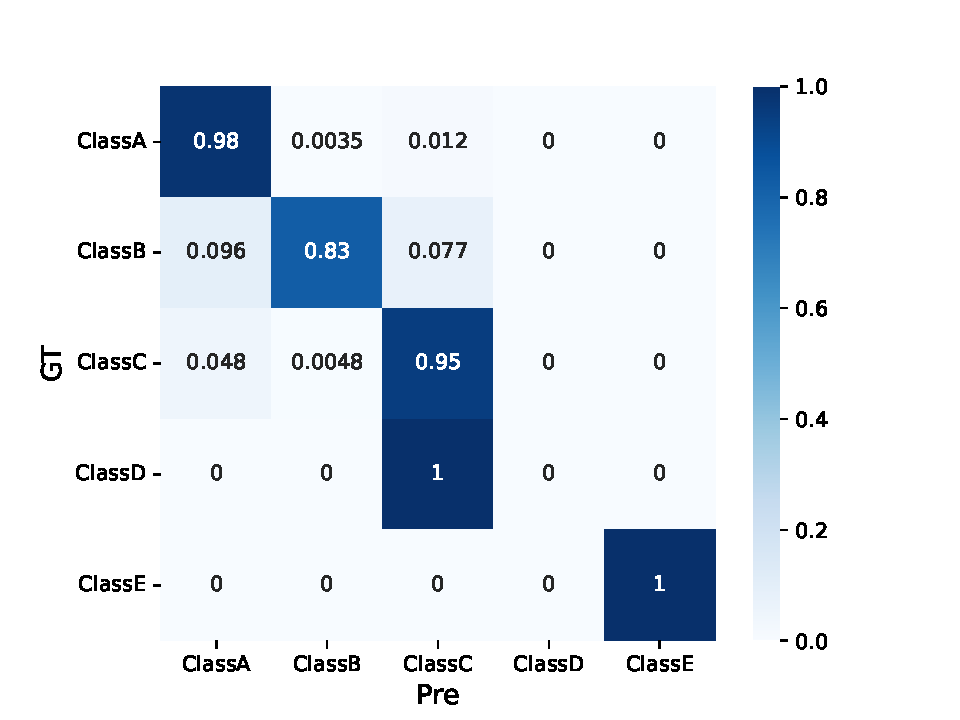
\includegraphics[keepaspectratio, scale=0.35]{images/deepimfam_confusion_matrix_ratio.pdf}
          \caption{もとのデータ}
        \end{figure}
      \end{column}
      \begin{column}{0.48\textwidth}
        \begin{figure}[H]
          \centering
          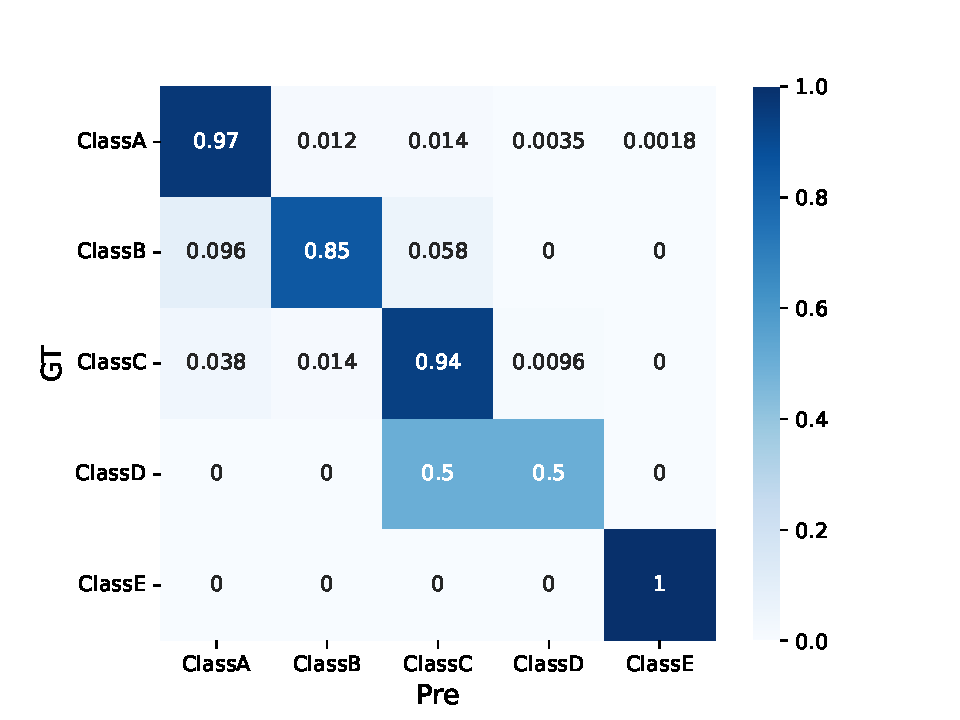
\includegraphics[keepaspectratio, scale=0.35]{images/deepimfam_augmentation_confusion_matrix_ratio.pdf}
          \caption{水増しデータ}
        \end{figure}
      \end{column}
    \end{columns}
  \end{frame}
\end{document}

